%\chapter{Cap\'{\i}tulo 3}
\chapter{Solution Proposal}

In this section we propose one element as an extension for Preconceptual Schemas(PS) which aid the understanding of diverse elements in the oil reservoir simulation domain. In addition, we present further description of the concepts stated in the theoretical framework, with their respective representation in the elaborated PS.
\\
This section is structured as follows: in section \ref{sec:PSNew} we present the added elements to PS and their usage in our represented domain. In section \ref{sec:PS_EOR} we propose the representation of structural and dynamical behavior of each developed concept in the theoretical framework using PS.

\section{Added elements to Preconceptual Schemas}\label{sec:PSNew}
\subsection{Analyst defined subroutines}\label{sec:PS_ADS}
Analyst defined subroutines are analyst defined functions as proposed by (ref Calle) without the return argument. They use global elements and parameters of the subroutine definition. They are defined for re-using dynamical behavior elements which appear more than once in the PS. Names of both subroutines and functions must differ from operators predefined in the PS. Graphic symbol used for subroutines is the same as used for operators and functions. In figure \# we present graphical representation of analyst defined subroutines.

\section{Conceptualization}
%
\subsection{Mesh}
%
\subsection{Rock}
%
\subsection{Phase}
%
\subsection{Inter-phase interaction}
%
\subsection{Component}
%
\subsection{Equlibrium Relation}
%
\subsection{Well}

\section{PS Representation of Enhanced Oil Recovery Simulation}\label{sec:PS_EOR}
In this section we propose a PS representation for enhanced oil recovery simulation, we couple a black oil model discretized using finite volumes method with the theoretical framework developed the previous chapter. We mapped each term in the resultant equations to their respective concepts and how they are linked together. The complete representation is shown in \ref{fig:PSComplete}.\\
\begin{figure}[h]
\centering%
\includegraphics[width=0.9\linewidth]{Kap4/MultifasicoSinPozos.pdf}%
\caption{Complete PS Representation for EOR Processes} \label{fig:PSComplete}
\end{figure}

The rest of this section is as follows: In section \ref{sec:PS_Mesh} we present the Mesh concept as a collection of cells with additional elements needed for calculating the attributes of each cell. Furthermore, we develop the dynamical relationship ``Geomodeler defines Mesh'' as an interaction of the role ``Geomodeler'' with atomic\footnote{atomic as is stated by \cite{AG01} (Aca debe ir Zapata)} dynamical relationships. In section \ref{sec:PS_Rock} we present the Rock concept with its attributes and initial characterization. In section \ref{sec:PS_Phase} ... In section \ref{sec:PS_Interphase} ... In section \ref{sec:PS_Equilibrium} we define the partition coefficients as relations between two phases, one contributing mass and another receiving mass in the mass balance equation. In section \ref{sec:PS_Well}  

\subsection{Mesh}\label{sec:PS_Mesh}

We propose a representation of a mesh as a collection of cells which are represented likewise. collection of faces plus their respective attributes. This representation accounts for orthogonal cartesian meshes. Those are generated using the number of cells in each axis or direction, the thickness and top for each cell. Nevertheless, the thickness is only needed for the number of cells defined in every axis, because we work with regular meshes. Therefore the rest of the cells will have the same thickness.
\\
The top of the mesh is required for the first XY plane, and needs to be filled with the depths of each cell in that plane, the rest of the cells are calculated using the depth of the first plane.

The representation stated for Mesh only accounts for orthogonal cartesian meshes, which can be generated with information about number of cells in each axis, their thickness and tops. A (The information above is inserted by a) Geomodeler with defines the mesh by inserting for each axis the number of cells and the thickness for cells in that direction. Once 
\ref{fig:Mesh}.\\
\begin{figure}[h]
	\centering%
	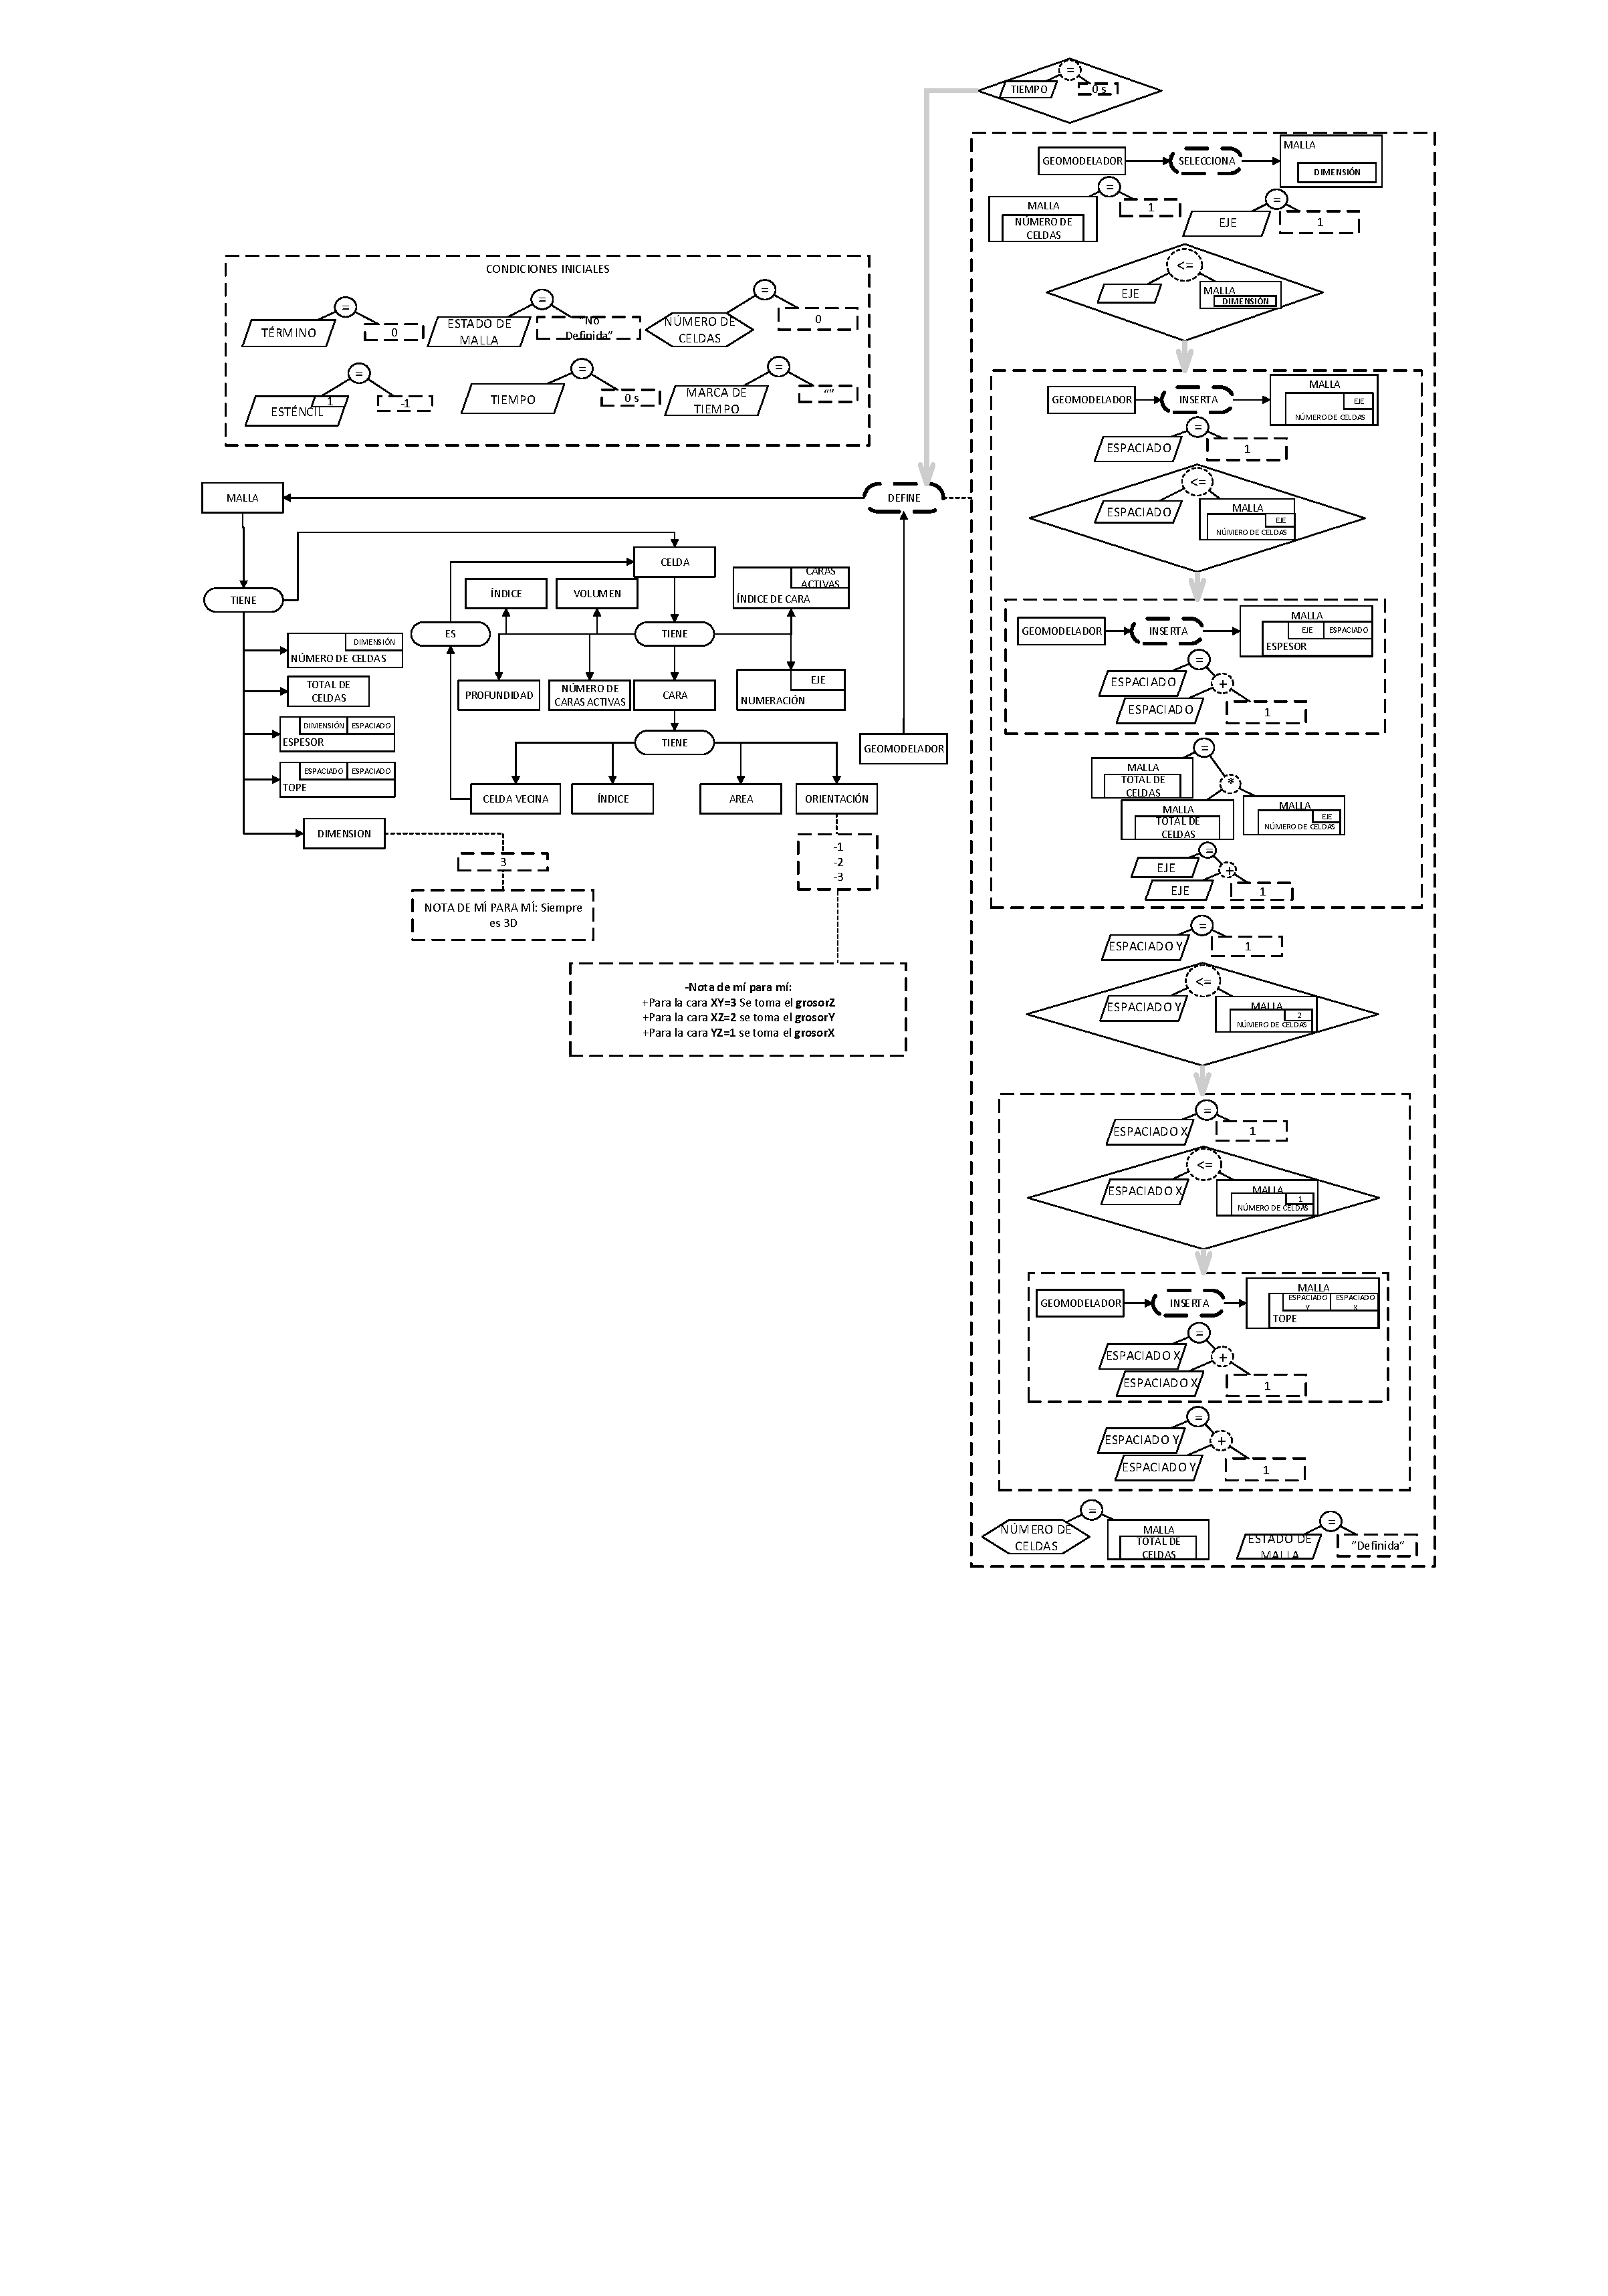
\includegraphics[width=0.9\linewidth]{Kap4/Mesh.pdf}%
	\caption{Mesh definition.} \label{fig:Mesh}
\end{figure}

\subsection{Rock}\label{sec:PS_Rock}
\ref{fig:Rock}.\\
\begin{figure}[h]
	\centering%
	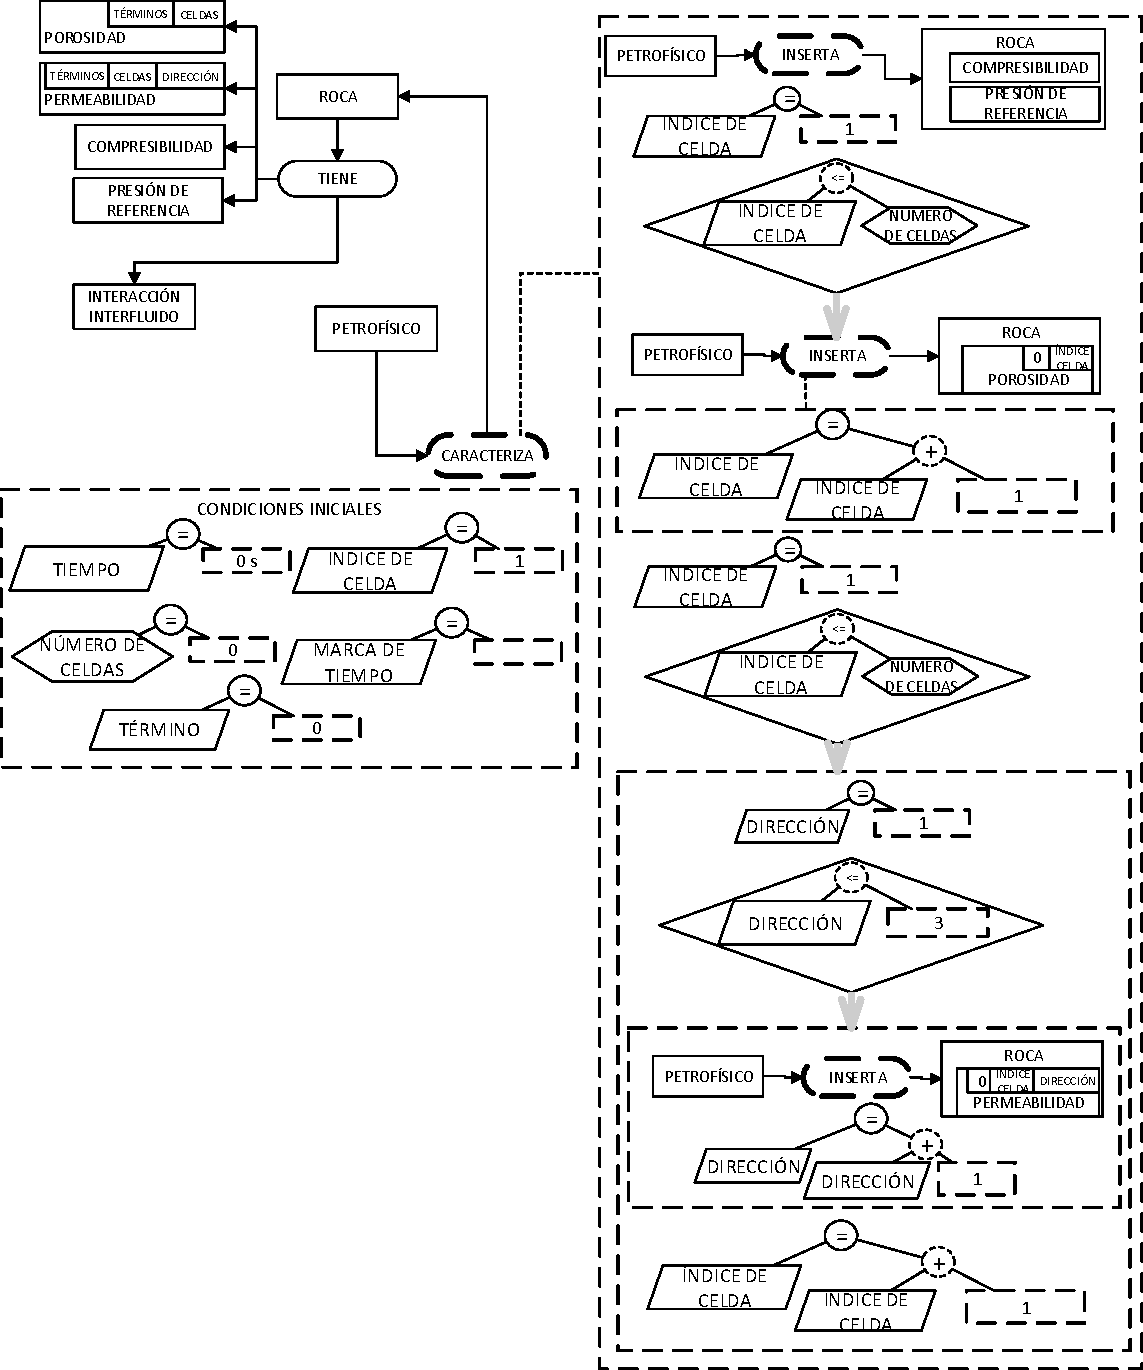
\includegraphics[width=0.9\linewidth]{Kap4/Rock.pdf}%
	\caption{Fluid Characterization.} \label{fig:Rock}
\end{figure}
\subsection{Phase}\label{sec:PS_Phase}

\ref{fig:Fluid}.\\
\begin{figure}[h]
	\centering%
	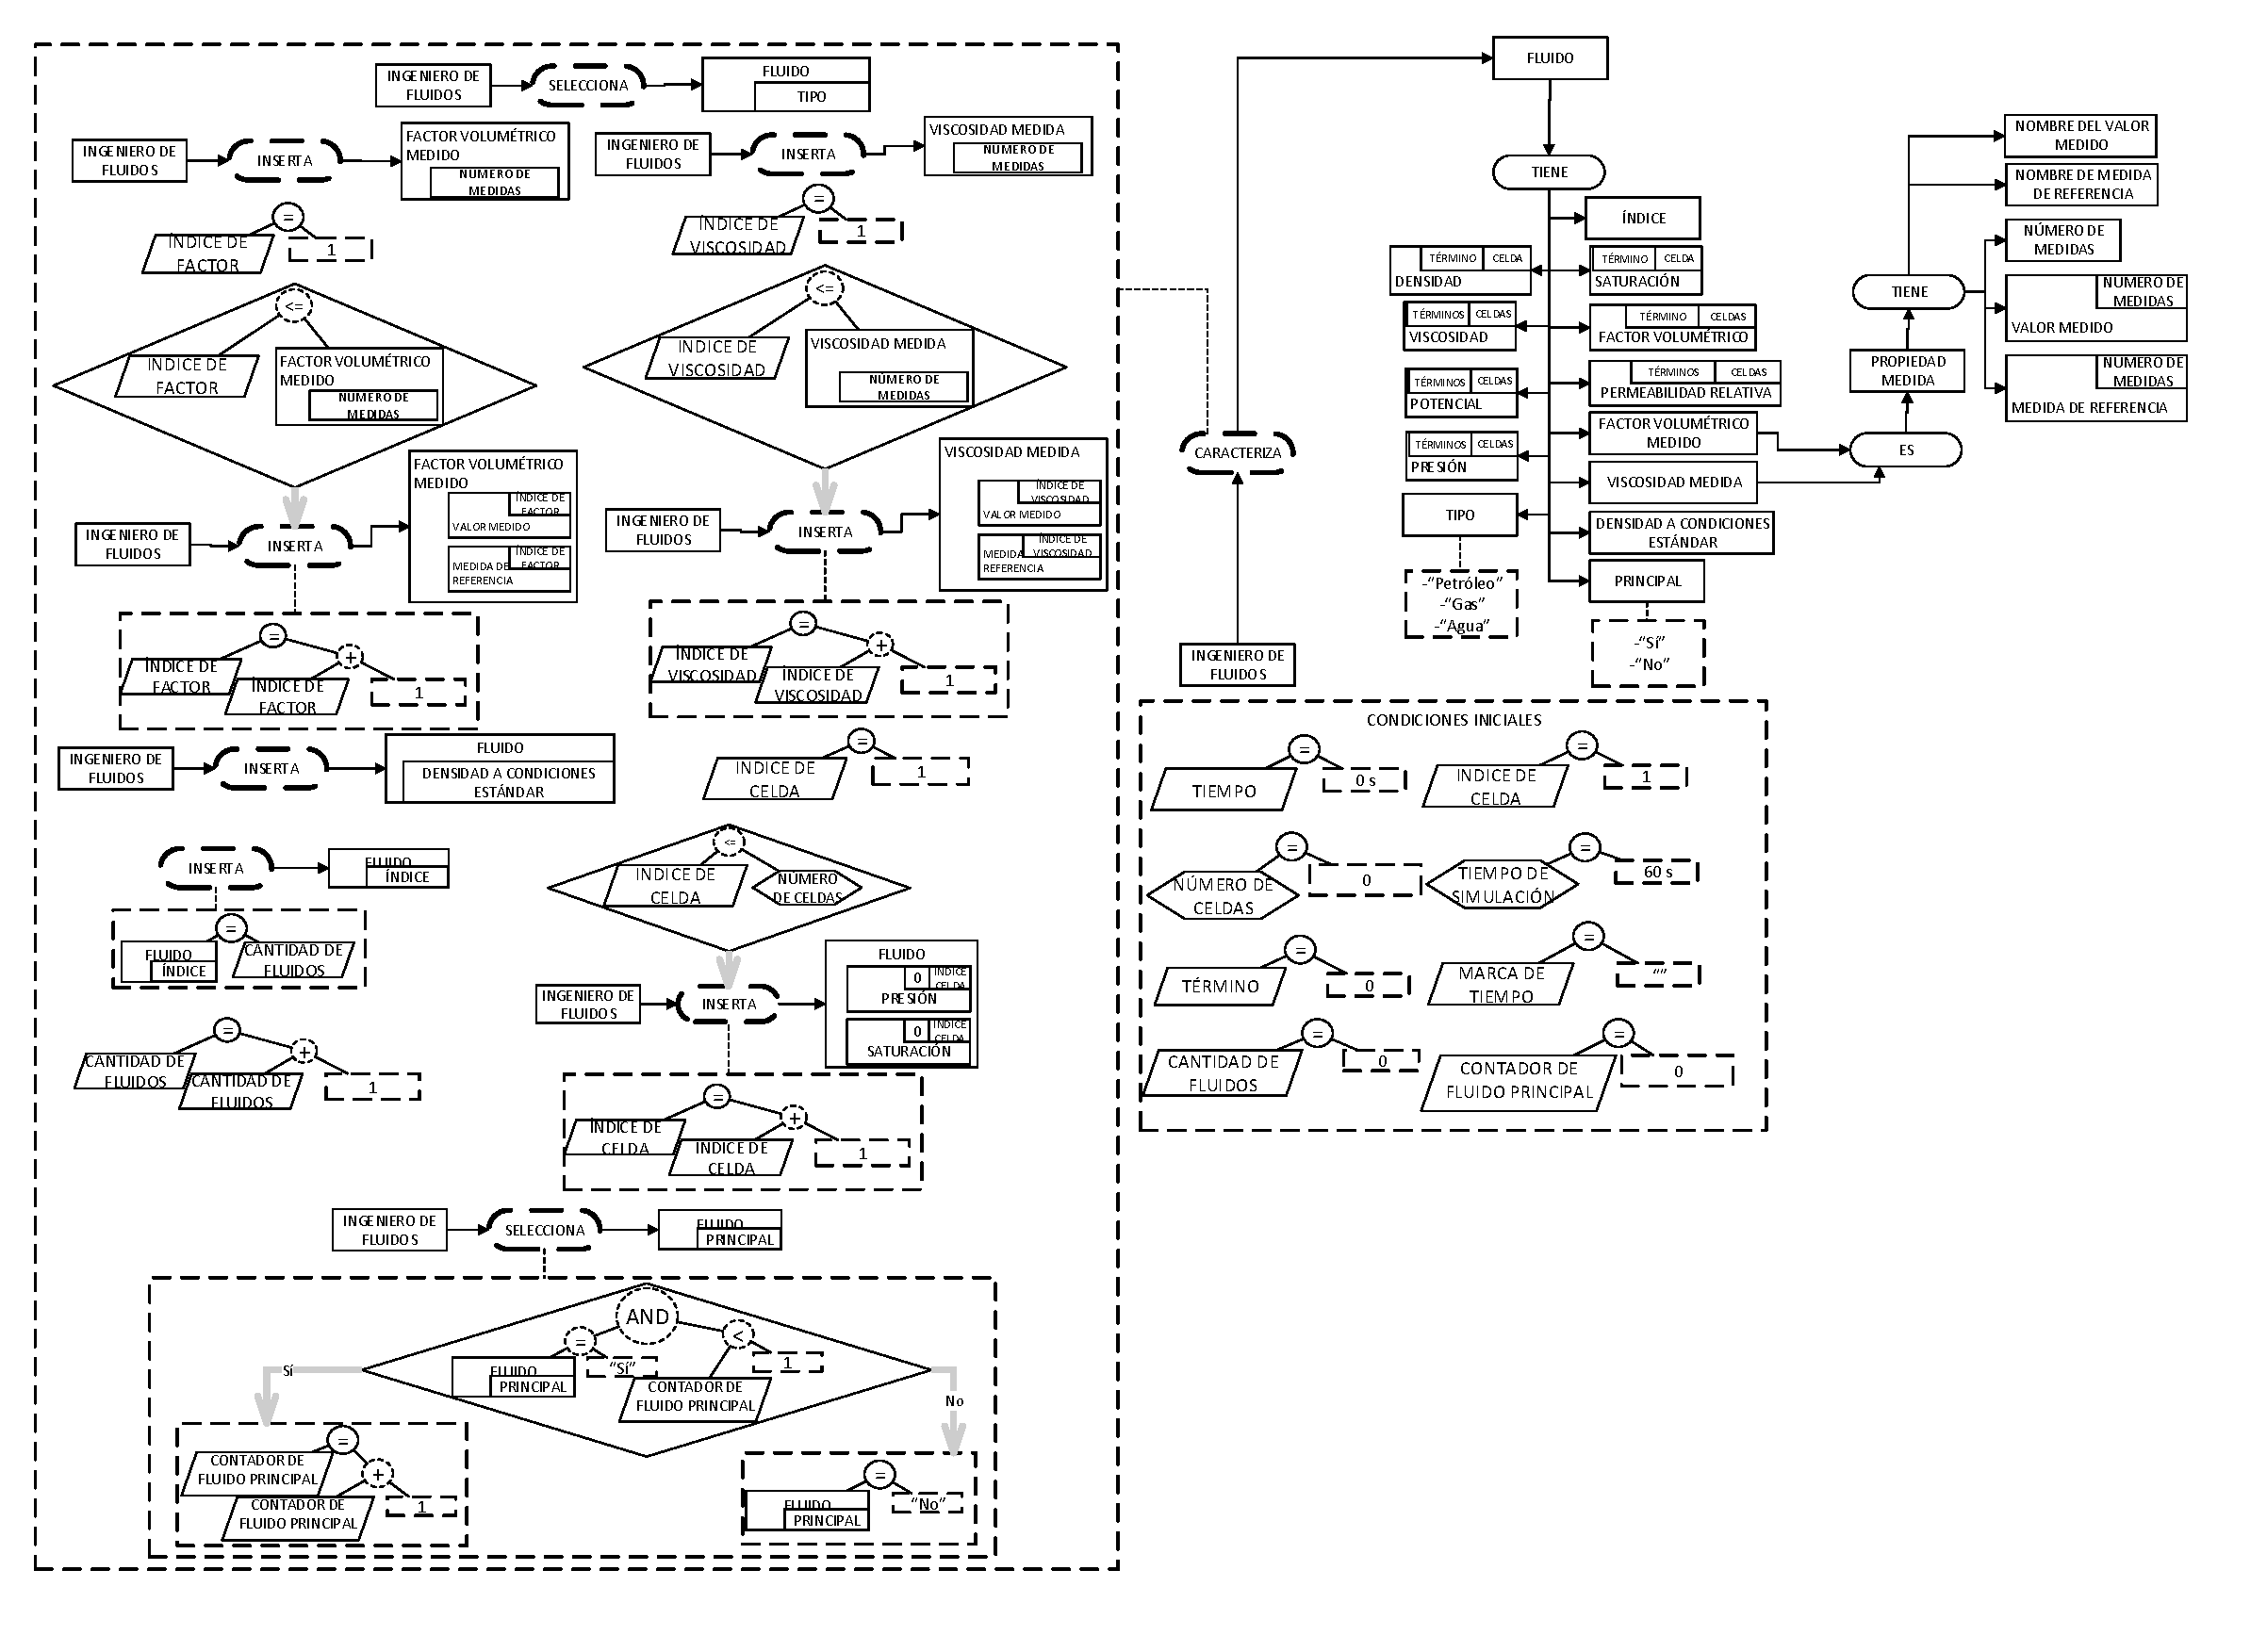
\includegraphics[width=0.9\linewidth]{Kap4/Fluid.pdf}%
	\caption{Fluid Characterization.} \label{fig:Fluid}
\end{figure}

\subsection{Inter-phase interaction}\label{sec:PS_Interphase}

%\subsection{Component}\label{sec:PS_Component} % This could be changed to Chemical

\subsection{Equilibrium Relation}\label{sec:PS_Equilibrium}

\subsection{Well}\label{sec:PS_Well}

%includefigure{Graphical Representation of subroutine}

%includegraphic{Code Translation}

%Se deben incluir tantos cap\'{\i}tulos como se requieran; sin embargo, se recomienda que la tesis  o trabajo de investigaci\'{o}n tenga un m\'{\i}nimo 3 cap\'{\i}tulos y m\'{a}ximo de 6 cap\'{\i}tulos (incluyendo las conclusiones).\\